\section{Maps}%
\label{sec:maps}

\begin{frame}
	\frametitle{Maps}
	
	\begin{center}
		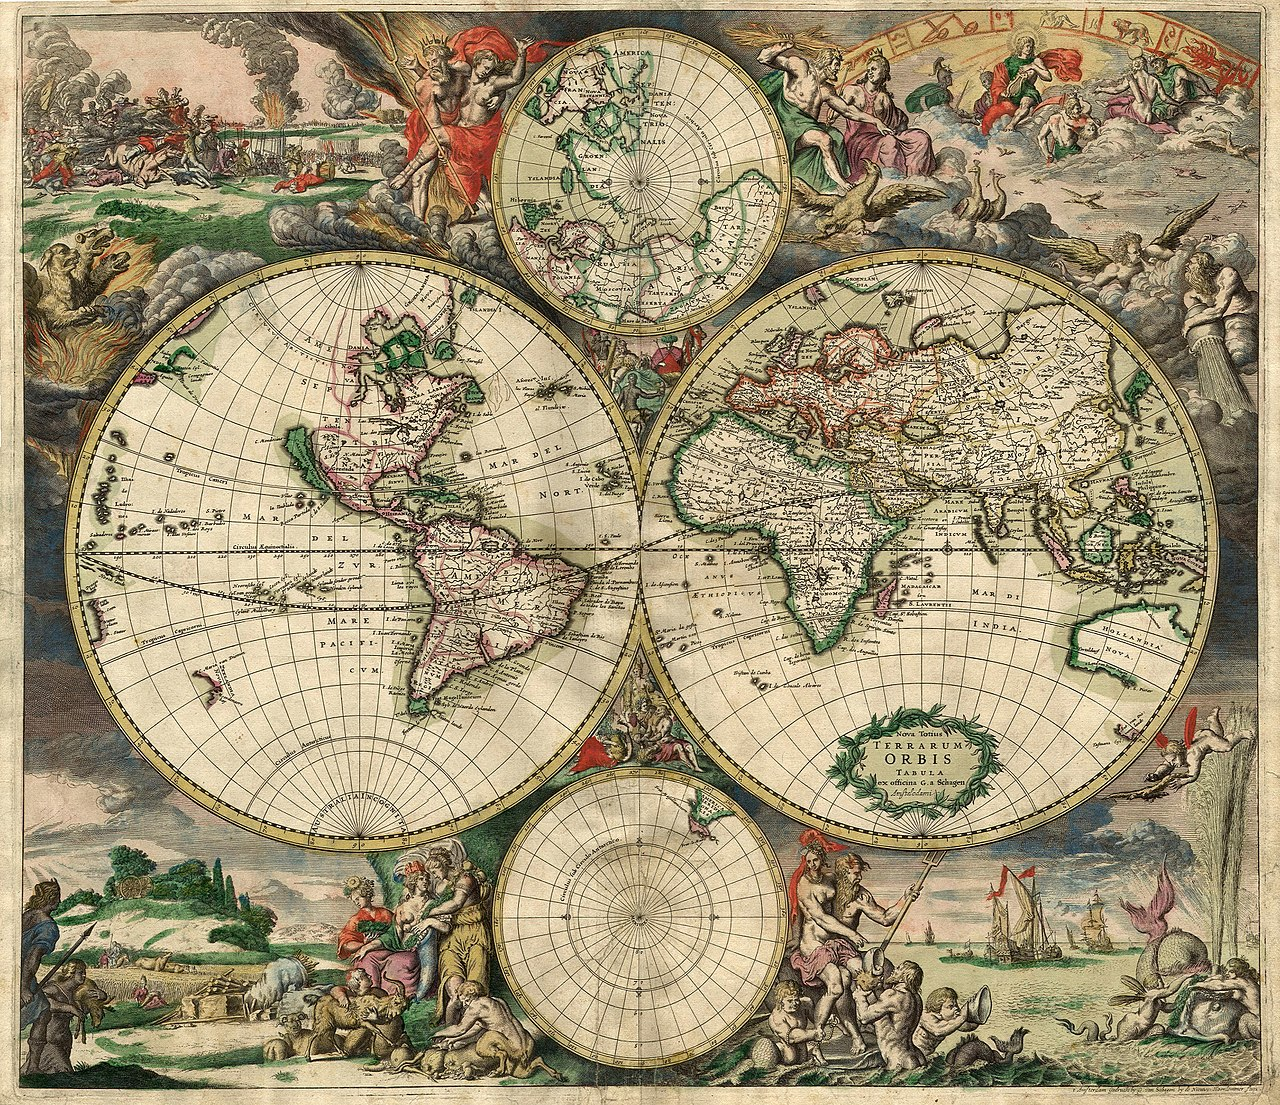
\includegraphics[width=0.5\textwidth]{figures/world_map.JPG}\\
		\hspace*{15pt}\hbox{\scriptsize Image By:\thinspace{\itshape Gerard van Schagen}}
		%https://commons.wikimedia.org/wiki/File:World_Map_1689.JPG
	\end{center}
\end{frame}

\begin{frame}
	\frametitle{The map ADT}
	
		\begin{block}{The map ADT}
			Maps work on \textit{key-value} pairs, usually denoted as tuples: $(k,v)$.
			\pause
			\begin{itemize}
				\item \texttt{M.size()} (or \texttt{len(M)}) to get the number of tuples in the map.
					\pause
				\item \texttt{M.get(k)} (or \texttt{M[k]}) to retrieve the value for key $k$.
				\item \texttt{M.put(k,v)} (or \texttt{M[k] = v}) to set the value for key $k$ to $v$.
					\pause
				\item \texttt{M.remove(k)} (or \texttt{del M[k]}) to remove the tuple with key $k$.
					\pause
				\item \texttt{M.contains(k)} (or \texttt{k in M}) to determine if there is tuple with key $k$.
			\end{itemize}
		\end{block}	
\end{frame}

\begin{frame}
	\frametitle{A naive implementation}
	\framesubtitle{Listing a map}

	\begin{questionblock}{Why not just use a list?}
		If we use a list to implement the map where we just throw in all the tuples, what would the time complexity
		of the functions \texttt{get}, \texttt{remove}, \texttt{contains} be?
		\pause
		\begin{enumerate}[A.]
			\item $\Theta(1)$
			\item $\Theta(\log n)$
			\item $\Theta(n)$
			\item $\Theta(n^2)$
			\item I don't know
		\end{enumerate}
	\end{questionblock}
	\pause
	\begin{alertblock}{Not so great}
		All would take linear time! \\
		We would just have to check all the objects every time!
	\end{alertblock}
\end{frame}

\begin{frame}
	\frametitle{Can we do better?}
	\begin{questionblock}{Can we do better?} 
		Can we do better, and if so how?
	\end{questionblock}	
	\pause
	\begin{answerblock}{Yes!}
		How about we try to use an array-based structure where the key determines the index?\\
		\pause
		This allows for $\Theta(1)$ operations for getting, removing or checking an item!
	\end{answerblock}
	\pause
	\begin{alertblock}{But...}
		But what if the key is not integer?
	\end{alertblock}
\end{frame}
